\documentclass[12pt]{article}
\usepackage[paperwidth=50cm,paperheight=100cm,margin=1cm]{geometry}
\usepackage{xeCJK}
\usepackage{fontspec}
\usepackage{graphicx}
\usepackage{xcolor}
\usepackage{indentfirst}
\usepackage{tikz}
\usepackage{pgfplots}
\usepackage{amssymb}
\usepackage{amsthm}
\usepackage{amsmath}
\usepackage{fancyhdr}
\usepackage{tabularx}
\usepackage{hyperref}
\usepackage{xurl}
\usepackage{ulem}
\usepackage{version}
\usepackage{thmtools}
\usepackage{qtree}
\usepackage{algorithm}
\usepackage{algpseudocode}
\usepackage{mathtools}
\usepackage[shortlabels]{enumitem}
%\usepackage{minted}
\usepackage{mdframed}
\usepackage{lipsum}

\XeTeXlinebreaklocale "zh"
\XeTeXlinebreakskip = 0pt plus 1pt

\setCJKmainfont{Noto Sans CJK TC}
\setmonofont{Source Code Pro}
\usetikzlibrary{arrows,decorations.markings,decorations.pathreplacing}
\pagestyle{empty}

\tikzstyle {graph node} = [circle, draw, minimum width=1cm]
\tikzset{edge/.style = {decoration={markings,mark=at position 1 with %
            {\arrow[scale=2,>=stealth]{>}}},postaction={decorate}}}

\renewcommand{\baselinestretch}{1.3}

\newtheoremstyle{owo}% name of the style to be used
  {10pt}% measure of space to leave above the theorem. E.g.: 3pt
  {10pt}% measure of space to leave below the theorem. E.g.: 3pt
  {}% name of font to use in the body of the theorem
  {}% measure of space to indent
  {\bfseries}% name of head font
  { }% punctuation between head and body
  { }% space after theorem head; " " = normal interword space
  {\thmname{#1}\thmnumber{ #2}.\thmnote{ (#3)}}

\theoremstyle{owo}
\newtheorem{Theorem}{Theorem}
\newtheorem{Lemma}{Lemma}
\newtheorem{Observation}{Observation}
\newtheorem{Corollary}{Corollary}
\newtheorem*{Proof}{Proof}

\DeclareMathOperator*{\argmin}{argmin}

\hypersetup{
    %colorlinks=true,
    }

%\usemintedstyle{vs}
%\renewcommand{\theFancyVerbLine}{\ttfamily\normalsize\arabic{FancyVerbLine}}
%\newenvironment{Code}[1]{~\vspace{-15pt}\VerbatimEnvironment\begin{minted}[bgcolor=black!5!white, breaklines, linenos]{#1}}{\end{minted}}

\newcommand{\Inline}{\mintinline[bgcolor=black!5!white, breaklines]{text}}

\newmdenv[topline=false, bottomline=false, rightline=false, linewidth=3pt, linecolor=black!10!white]{Quotemd}
\newenvironment{Quote}{~\vspace{-15pt}\begin{Quotemd}}{\end{Quotemd}}

\begin{document}

\setlist[enumerate]{itemsep=0pt, parsep=0pt, topsep=0pt}
\setlist[itemize]{itemsep=0pt, parsep=0pt, topsep=0pt}

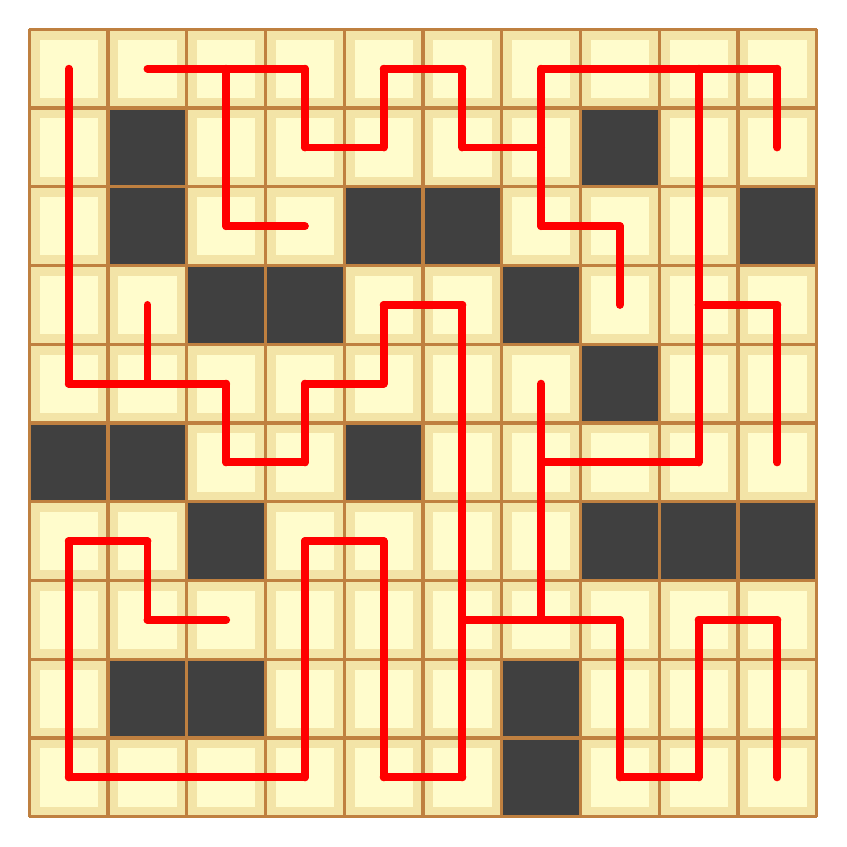
\begin{tikzpicture}[x={(0,-1cm)}, y={(1cm,0)}]

    \draw[fill=yellow!25!white!80!brown] (0.5, 0.5) rectangle ++(10, 10);

\draw[fill=yellow!20!white, draw=none] (0.63,0.63) rectangle ++ (0.74,0.74);
\draw[fill=yellow!20!white, draw=none] (0.63,1.63) rectangle ++ (0.74,0.74);
\draw[fill=yellow!20!white, draw=none] (0.63,2.63) rectangle ++ (0.74,0.74);
\draw[fill=yellow!20!white, draw=none] (0.63,3.63) rectangle ++ (0.74,0.74);
\draw[fill=yellow!20!white, draw=none] (0.63,4.63) rectangle ++ (0.74,0.74);
\draw[fill=yellow!20!white, draw=none] (0.63,5.63) rectangle ++ (0.74,0.74);
\draw[fill=yellow!20!white, draw=none] (0.63,6.63) rectangle ++ (0.74,0.74);
\draw[fill=yellow!20!white, draw=none] (0.63,7.63) rectangle ++ (0.74,0.74);
\draw[fill=yellow!20!white, draw=none] (0.63,8.63) rectangle ++ (0.74,0.74);
\draw[fill=yellow!20!white, draw=none] (0.63,9.63) rectangle ++ (0.74,0.74);
\draw[fill=yellow!20!white, draw=none] (1.63,0.63) rectangle ++ (0.74,0.74);
\draw[fill=black!50!gray, draw=none] (1.5,1.5) rectangle ++ (1,1);
\draw[fill=yellow!20!white, draw=none] (1.63,2.63) rectangle ++ (0.74,0.74);
\draw[fill=yellow!20!white, draw=none] (1.63,3.63) rectangle ++ (0.74,0.74);
\draw[fill=yellow!20!white, draw=none] (1.63,4.63) rectangle ++ (0.74,0.74);
\draw[fill=yellow!20!white, draw=none] (1.63,5.63) rectangle ++ (0.74,0.74);
\draw[fill=yellow!20!white, draw=none] (1.63,6.63) rectangle ++ (0.74,0.74);
\draw[fill=black!50!gray, draw=none] (1.5,7.5) rectangle ++ (1,1);
\draw[fill=yellow!20!white, draw=none] (1.63,8.63) rectangle ++ (0.74,0.74);
\draw[fill=yellow!20!white, draw=none] (1.63,9.63) rectangle ++ (0.74,0.74);
\draw[fill=yellow!20!white, draw=none] (2.63,0.63) rectangle ++ (0.74,0.74);
\draw[fill=black!50!gray, draw=none] (2.5,1.5) rectangle ++ (1,1);
\draw[fill=yellow!20!white, draw=none] (2.63,2.63) rectangle ++ (0.74,0.74);
\draw[fill=yellow!20!white, draw=none] (2.63,3.63) rectangle ++ (0.74,0.74);
\draw[fill=black!50!gray, draw=none] (2.5,4.5) rectangle ++ (1,1);
\draw[fill=black!50!gray, draw=none] (2.5,5.5) rectangle ++ (1,1);
\draw[fill=yellow!20!white, draw=none] (2.63,6.63) rectangle ++ (0.74,0.74);
\draw[fill=yellow!20!white, draw=none] (2.63,7.63) rectangle ++ (0.74,0.74);
\draw[fill=yellow!20!white, draw=none] (2.63,8.63) rectangle ++ (0.74,0.74);
\draw[fill=black!50!gray, draw=none] (2.5,9.5) rectangle ++ (1,1);
\draw[fill=yellow!20!white, draw=none] (3.63,0.63) rectangle ++ (0.74,0.74);
\draw[fill=yellow!20!white, draw=none] (3.63,1.63) rectangle ++ (0.74,0.74);
\draw[fill=black!50!gray, draw=none] (3.5,2.5) rectangle ++ (1,1);
\draw[fill=black!50!gray, draw=none] (3.5,3.5) rectangle ++ (1,1);
\draw[fill=yellow!20!white, draw=none] (3.63,4.63) rectangle ++ (0.74,0.74);
\draw[fill=yellow!20!white, draw=none] (3.63,5.63) rectangle ++ (0.74,0.74);
\draw[fill=black!50!gray, draw=none] (3.5,6.5) rectangle ++ (1,1);
\draw[fill=yellow!20!white, draw=none] (3.63,7.63) rectangle ++ (0.74,0.74);
\draw[fill=yellow!20!white, draw=none] (3.63,8.63) rectangle ++ (0.74,0.74);
\draw[fill=yellow!20!white, draw=none] (3.63,9.63) rectangle ++ (0.74,0.74);
\draw[fill=yellow!20!white, draw=none] (4.63,0.63) rectangle ++ (0.74,0.74);
\draw[fill=yellow!20!white, draw=none] (4.63,1.63) rectangle ++ (0.74,0.74);
\draw[fill=yellow!20!white, draw=none] (4.63,2.63) rectangle ++ (0.74,0.74);
\draw[fill=yellow!20!white, draw=none] (4.63,3.63) rectangle ++ (0.74,0.74);
\draw[fill=yellow!20!white, draw=none] (4.63,4.63) rectangle ++ (0.74,0.74);
\draw[fill=yellow!20!white, draw=none] (4.63,5.63) rectangle ++ (0.74,0.74);
\draw[fill=yellow!20!white, draw=none] (4.63,6.63) rectangle ++ (0.74,0.74);
\draw[fill=black!50!gray, draw=none] (4.5,7.5) rectangle ++ (1,1);
\draw[fill=yellow!20!white, draw=none] (4.63,8.63) rectangle ++ (0.74,0.74);
\draw[fill=yellow!20!white, draw=none] (4.63,9.63) rectangle ++ (0.74,0.74);
\draw[fill=black!50!gray, draw=none] (5.5,0.5) rectangle ++ (1,1);
\draw[fill=black!50!gray, draw=none] (5.5,1.5) rectangle ++ (1,1);
\draw[fill=yellow!20!white, draw=none] (5.63,2.63) rectangle ++ (0.74,0.74);
\draw[fill=yellow!20!white, draw=none] (5.63,3.63) rectangle ++ (0.74,0.74);
\draw[fill=black!50!gray, draw=none] (5.5,4.5) rectangle ++ (1,1);
\draw[fill=yellow!20!white, draw=none] (5.63,5.63) rectangle ++ (0.74,0.74);
\draw[fill=yellow!20!white, draw=none] (5.63,6.63) rectangle ++ (0.74,0.74);
\draw[fill=yellow!20!white, draw=none] (5.63,7.63) rectangle ++ (0.74,0.74);
\draw[fill=yellow!20!white, draw=none] (5.63,8.63) rectangle ++ (0.74,0.74);
\draw[fill=yellow!20!white, draw=none] (5.63,9.63) rectangle ++ (0.74,0.74);
\draw[fill=yellow!20!white, draw=none] (6.63,0.63) rectangle ++ (0.74,0.74);
\draw[fill=yellow!20!white, draw=none] (6.63,1.63) rectangle ++ (0.74,0.74);
\draw[fill=black!50!gray, draw=none] (6.5,2.5) rectangle ++ (1,1);
\draw[fill=yellow!20!white, draw=none] (6.63,3.63) rectangle ++ (0.74,0.74);
\draw[fill=yellow!20!white, draw=none] (6.63,4.63) rectangle ++ (0.74,0.74);
\draw[fill=yellow!20!white, draw=none] (6.63,5.63) rectangle ++ (0.74,0.74);
\draw[fill=yellow!20!white, draw=none] (6.63,6.63) rectangle ++ (0.74,0.74);
\draw[fill=black!50!gray, draw=none] (6.5,7.5) rectangle ++ (1,1);
\draw[fill=black!50!gray, draw=none] (6.5,8.5) rectangle ++ (1,1);
\draw[fill=black!50!gray, draw=none] (6.5,9.5) rectangle ++ (1,1);
\draw[fill=yellow!20!white, draw=none] (7.63,0.63) rectangle ++ (0.74,0.74);
\draw[fill=yellow!20!white, draw=none] (7.63,1.63) rectangle ++ (0.74,0.74);
\draw[fill=yellow!20!white, draw=none] (7.63,2.63) rectangle ++ (0.74,0.74);
\draw[fill=yellow!20!white, draw=none] (7.63,3.63) rectangle ++ (0.74,0.74);
\draw[fill=yellow!20!white, draw=none] (7.63,4.63) rectangle ++ (0.74,0.74);
\draw[fill=yellow!20!white, draw=none] (7.63,5.63) rectangle ++ (0.74,0.74);
\draw[fill=yellow!20!white, draw=none] (7.63,6.63) rectangle ++ (0.74,0.74);
\draw[fill=yellow!20!white, draw=none] (7.63,7.63) rectangle ++ (0.74,0.74);
\draw[fill=yellow!20!white, draw=none] (7.63,8.63) rectangle ++ (0.74,0.74);
\draw[fill=yellow!20!white, draw=none] (7.63,9.63) rectangle ++ (0.74,0.74);
\draw[fill=yellow!20!white, draw=none] (8.63,0.63) rectangle ++ (0.74,0.74);
\draw[fill=black!50!gray, draw=none] (8.5,1.5) rectangle ++ (1,1);
\draw[fill=black!50!gray, draw=none] (8.5,2.5) rectangle ++ (1,1);
\draw[fill=yellow!20!white, draw=none] (8.63,3.63) rectangle ++ (0.74,0.74);
\draw[fill=yellow!20!white, draw=none] (8.63,4.63) rectangle ++ (0.74,0.74);
\draw[fill=yellow!20!white, draw=none] (8.63,5.63) rectangle ++ (0.74,0.74);
\draw[fill=black!50!gray, draw=none] (8.5,6.5) rectangle ++ (1,1);
\draw[fill=yellow!20!white, draw=none] (8.63,7.63) rectangle ++ (0.74,0.74);
\draw[fill=yellow!20!white, draw=none] (8.63,8.63) rectangle ++ (0.74,0.74);
\draw[fill=yellow!20!white, draw=none] (8.63,9.63) rectangle ++ (0.74,0.74);
\draw[fill=yellow!20!white, draw=none] (9.63,0.63) rectangle ++ (0.74,0.74);
\draw[fill=yellow!20!white, draw=none] (9.63,1.63) rectangle ++ (0.74,0.74);
\draw[fill=yellow!20!white, draw=none] (9.63,2.63) rectangle ++ (0.74,0.74);
\draw[fill=yellow!20!white, draw=none] (9.63,3.63) rectangle ++ (0.74,0.74);
\draw[fill=yellow!20!white, draw=none] (9.63,4.63) rectangle ++ (0.74,0.74);
\draw[fill=yellow!20!white, draw=none] (9.63,5.63) rectangle ++ (0.74,0.74);
\draw[fill=black!50!gray, draw=none] (9.5,6.5) rectangle ++ (1,1);
\draw[fill=yellow!20!white, draw=none] (9.63,7.63) rectangle ++ (0.74,0.74);
\draw[fill=yellow!20!white, draw=none] (9.63,8.63) rectangle ++ (0.74,0.74);
\draw[fill=yellow!20!white, draw=none] (9.63,9.63) rectangle ++ (0.74,0.74);
\foreach \x in {0,...,10} {
\draw[very thick, brown] (\x + 0.5, 0.5) -- (\x + 0.5, 10.5);\draw[very thick, brown] (0.5, \x + 0.5) -- (10.5, \x + 0.5);
}
\draw[color=red, line width=1mm, line cap=round](1,1) -- (2,1);
\draw[color=red, line width=1mm, line cap=round](2,1) -- (3,1);
\draw[color=red, line width=1mm, line cap=round](3,1) -- (4,1);
\draw[color=red, line width=1mm, line cap=round](4,1) -- (5,1);
\draw[color=red, line width=1mm, line cap=round](5,1) -- (5,2);
\draw[color=red, line width=1mm, line cap=round](5,2) -- (4,2);
\draw[color=red, line width=1mm, line cap=round](5,2) -- (5,3);
\draw[color=red, line width=1mm, line cap=round](5,3) -- (6,3);
\draw[color=red, line width=1mm, line cap=round](6,3) -- (6,4);
\draw[color=red, line width=1mm, line cap=round](6,4) -- (5,4);
\draw[color=red, line width=1mm, line cap=round](5,4) -- (5,5);
\draw[color=red, line width=1mm, line cap=round](5,5) -- (4,5);
\draw[color=red, line width=1mm, line cap=round](4,5) -- (4,6);
\draw[color=red, line width=1mm, line cap=round](4,6) -- (5,6);
\draw[color=red, line width=1mm, line cap=round](5,6) -- (6,6);
\draw[color=red, line width=1mm, line cap=round](6,6) -- (7,6);
\draw[color=red, line width=1mm, line cap=round](7,6) -- (8,6);
\draw[color=red, line width=1mm, line cap=round](8,6) -- (9,6);
\draw[color=red, line width=1mm, line cap=round](9,6) -- (10,6);
\draw[color=red, line width=1mm, line cap=round](10,6) -- (10,5);
\draw[color=red, line width=1mm, line cap=round](10,5) -- (9,5);
\draw[color=red, line width=1mm, line cap=round](9,5) -- (8,5);
\draw[color=red, line width=1mm, line cap=round](8,5) -- (7,5);
\draw[color=red, line width=1mm, line cap=round](7,5) -- (7,4);
\draw[color=red, line width=1mm, line cap=round](7,4) -- (8,4);
\draw[color=red, line width=1mm, line cap=round](8,4) -- (9,4);
\draw[color=red, line width=1mm, line cap=round](9,4) -- (10,4);
\draw[color=red, line width=1mm, line cap=round](10,4) -- (10,3);
\draw[color=red, line width=1mm, line cap=round](10,3) -- (10,2);
\draw[color=red, line width=1mm, line cap=round](10,2) -- (10,1);
\draw[color=red, line width=1mm, line cap=round](10,1) -- (9,1);
\draw[color=red, line width=1mm, line cap=round](9,1) -- (8,1);
\draw[color=red, line width=1mm, line cap=round](8,1) -- (7,1);
\draw[color=red, line width=1mm, line cap=round](7,1) -- (7,2);
\draw[color=red, line width=1mm, line cap=round](7,2) -- (8,2);
\draw[color=red, line width=1mm, line cap=round](8,2) -- (8,3);
\draw[color=red, line width=1mm, line cap=round](8,6) -- (8,7);
\draw[color=red, line width=1mm, line cap=round](8,7) -- (7,7);
\draw[color=red, line width=1mm, line cap=round](7,7) -- (6,7);
\draw[color=red, line width=1mm, line cap=round](6,7) -- (5,7);
\draw[color=red, line width=1mm, line cap=round](6,7) -- (6,8);
\draw[color=red, line width=1mm, line cap=round](6,8) -- (6,9);
\draw[color=red, line width=1mm, line cap=round](6,9) -- (5,9);
\draw[color=red, line width=1mm, line cap=round](5,9) -- (4,9);
\draw[color=red, line width=1mm, line cap=round](4,9) -- (3,9);
\draw[color=red, line width=1mm, line cap=round](3,9) -- (2,9);
\draw[color=red, line width=1mm, line cap=round](2,9) -- (1,9);
\draw[color=red, line width=1mm, line cap=round](1,9) -- (1,8);
\draw[color=red, line width=1mm, line cap=round](1,8) -- (1,7);
\draw[color=red, line width=1mm, line cap=round](1,7) -- (2,7);
\draw[color=red, line width=1mm, line cap=round](2,7) -- (3,7);
\draw[color=red, line width=1mm, line cap=round](3,7) -- (3,8);
\draw[color=red, line width=1mm, line cap=round](3,8) -- (4,8);
\draw[color=red, line width=1mm, line cap=round](2,7) -- (2,6);
\draw[color=red, line width=1mm, line cap=round](2,6) -- (1,6);
\draw[color=red, line width=1mm, line cap=round](1,6) -- (1,5);
\draw[color=red, line width=1mm, line cap=round](1,5) -- (2,5);
\draw[color=red, line width=1mm, line cap=round](2,5) -- (2,4);
\draw[color=red, line width=1mm, line cap=round](2,4) -- (1,4);
\draw[color=red, line width=1mm, line cap=round](1,4) -- (1,3);
\draw[color=red, line width=1mm, line cap=round](1,3) -- (2,3);
\draw[color=red, line width=1mm, line cap=round](2,3) -- (3,3);
\draw[color=red, line width=1mm, line cap=round](3,3) -- (3,4);
\draw[color=red, line width=1mm, line cap=round](1,3) -- (1,2);
\draw[color=red, line width=1mm, line cap=round](1,9) -- (1,10);
\draw[color=red, line width=1mm, line cap=round](1,10) -- (2,10);
\draw[color=red, line width=1mm, line cap=round](4,9) -- (4,10);
\draw[color=red, line width=1mm, line cap=round](4,10) -- (5,10);
\draw[color=red, line width=1mm, line cap=round](5,10) -- (6,10);
\draw[color=red, line width=1mm, line cap=round](8,7) -- (8,8);
\draw[color=red, line width=1mm, line cap=round](8,8) -- (9,8);
\draw[color=red, line width=1mm, line cap=round](9,8) -- (10,8);
\draw[color=red, line width=1mm, line cap=round](10,8) -- (10,9);
\draw[color=red, line width=1mm, line cap=round](10,9) -- (9,9);
\draw[color=red, line width=1mm, line cap=round](9,9) -- (8,9);
\draw[color=red, line width=1mm, line cap=round](8,9) -- (8,10);
\draw[color=red, line width=1mm, line cap=round](8,10) -- (9,10);
\draw[color=red, line width=1mm, line cap=round](9,10) -- (10,10);

\end{tikzpicture}

\end{document}
